\section{Theory}

\subsection{Ball Grid Array PCB layout}

\acrshort{bga} refers to a packaging type used for surface mount \acrshort{ic}s. \acrshort{bga} packages feature all interconnects on the bottom of the package and allows for a higher number of connected pins than with pins on the edges of the package, see figure \ref{fig:clg255}.

\begin{figure}[H]
    \centering
    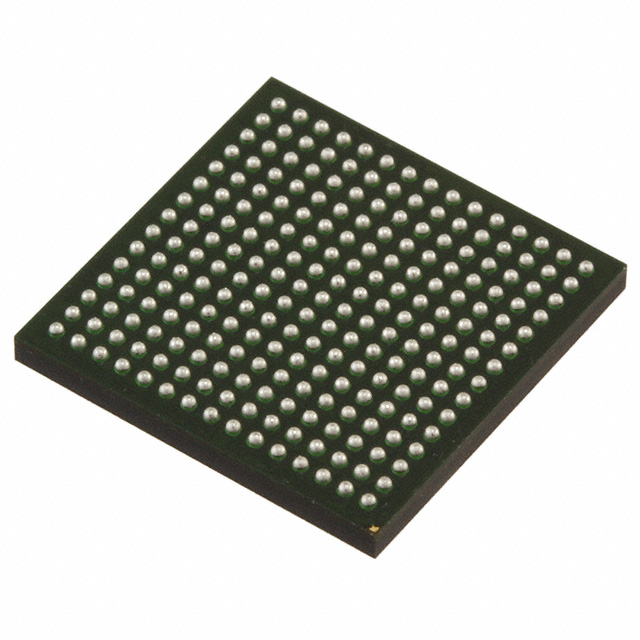
\includegraphics[width=.75\textwidth]{media/CLG225.JPG}
    \caption{CLG255, a 15-by-15 pin \acrshort{bga} package used by some \acrshort{soc}s in the Xilinx Zynq-7000 series. Illustration image taken from the XC7Z010-2CLG225I product page on www.digikey.com \cite{clg225}.}
    \label{fig:clg255}
\end{figure}

As the pins are hidden when the package is mounted on a \acrshort{pcb}, \acrshort{bga} packages must be soldered by other methods than classical hand-soldering. Reflow soldering is a popular method for soldering \acrshort{bga}'s where the entire package and adhering \acrshort{pcb} are heated to the point where all the solder melts. This is typically performed in a dedicated reflow soldering oven, but can also be performed using a hot-air gun or similar.


\subsection{CAN-FD}

The different embedded systems on the vehicle communicate with each other using \acrshort{canfd}. \acrfull{can} is a network bus developed by Bosch. It has been the de-facto standard communication platform for automotive applications since the mid-1990's. An improved version, \acrfull{canfd} was released by Bosh in 2012, it differs from \acrshort{can} in that the body of each message (called \emph{frames} for \acrshort{can}) are transmitted at a higher frequency than the header and the allowed frame size increases from 8 to 64 bytes. This is the communication bus currently used at Revolve NTNU.

\acrshort{can} and \acrshort{canfd} is a one-to-many bus system where each frame is given an identifier which determines the priority of the frame. When the bus is free, all connected devices can begin transmitting their frame, but the frame with the highest priority will take precedence on the bus. When a frame is transmitted on the bus, any connected device are able to read it. When the frame has successfully been transmitted the bus is again free and a new transmission can begin.

\subsubsection{CAN-FD bus utilization}

Almost all messages sent over the \acrshort{canfd} bus are sent at a regular interval. The size of the different messages are also known, this means that we know how long each message will occupy the bus for. These facts means that the frames on the bus can be modelled in the same way as tasks in a \acrfull{rms} system, known from real-time theory. This means the standard formula for utilization can be used when analyzing \acrshort{can} and \acrshort{canfd} buses. The equation for utilization $U$ on a bus is given in equation \ref{eq:utilization}. 

\begin{equation}
    U=\sum_{i=1}^N\frac{C_i}{T_i}
    \label{eq:utilization}
\end{equation}

$C_i$ is how long task $i$ takes to execute (execution time) and $T_i$ is how often the task is set to execute (execution period). In our case this is translated to the time frame $i$ is active on the bus and the period at which it should be transmitted. 


\subsubsection{Maximum utilization} \label{sec:max_util}

We can use the \emph{Utilization-based schedulability test} \cite{ttk4147} to determine whether all deadlines are met for a set of tasks. The criteria can be seen in equation \ref{eq:utilization_criteria}. It is important to note that this test is sufficient but not necessary. This means that a passing test guarantees all deadlines are met but a failing test does not guarantee missed deadlines.

\begin{equation}
    U=\sum_{i=1}^N\frac{C_i}{T_i}\leq N\left(2^\frac{1}{N}-1\right)
    \label{eq:utilization_criteria}
\end{equation}

$N$ denotes the number of different tasks being scheduled. Since the number of different messages on the CAN-FD buses is quite high, we might as well look at what happens to the criteria when $N$ goes towards infinity.

\begin{equation}
    \lim_{N\rightarrow\infty} N\left(2^\frac{1}{N}-1\right)=\ln{2}\approx 0.693
    \label{eq:utilization_criteria_calc}
\end{equation}

From equation \ref{eq:utilization_criteria_calc} we can deem that as long as the bus load on each of the \acrshort{canfd} buses are below 69.3\%, no messages are lost. This does of course not mean that the vehicle becomes unusable, figure \ref{fig:canfd_load} shows that the load was above the the limit for both buses, and the vehicle worked fine. The embedded systems are naturally made to be resilient to frame loss.

However, the limit serves as a good target for max bus load, and we will work towards lowering bus load to below this limit.

%The high load on the CAN-FD buses poses one of the big challenges with the current system. We want a mathematical model of the load on the CAN-FD buses which can tell us whether messages will be lost or not.


%\subsubsection{Rate-Monotonic Scheduling}

%As the messages sent over the CAN-FD buses are sent at a somewhat regular interval, the buses can be modeled as a rate-monotonic scheduled (RMS) system. This is a way to model the scheduling of software tasks when the tasks are run at a set interval and with a fixed execution time. We begin by looking at the equation for utilization used with RMS.

%Equation \ref{eq:utilization} shows how utilization is calculated for tasks, i.e. how much of the time that a task executes on a single core processor. 

\subsubsection{CAN-FD utilization}

From the \acrshort{rms} utilization equation we know that we need the execution time $C$ and period $T$ for each task. While the period for each CAN-FD message is easy to determine, the execution time takes slighly more effort.From now on we will call the execution time for a message $m$ the \emph{transmission time} and we will denote it $C_m$. For a standard \acrshort{can} message it would be sufficient to divide the number of bits in the message by the operating frequency of the bus. This is made slightly more difficult as \acrshort{canfd} operates on two different frequencies, one for arbitration (header) transmission and one for data transmission. We can split look at the total transmission time as a sum of the transmission time for each of the frequencies, see equation \ref{eq:canfd_cm}.  

\begin{equation}
    C_m=C_s+C_f
    \label{eq:canfd_cm}
\end{equation}

$C_s$ is the transmission time for the message header. It is independent of frame size and the calculation can be seen in equation \ref{eq:canfd_ts}.

\begin{equation}
    \begin{gathered}
        C_s=\frac{(SOF+ID+r1+IDE+EDL+r0+\frac{BRS}{2}+\frac{CRCdel}{2})\cdot1.2}{t_x}\\+\frac{ACK+DEL+EOF+IFS}{t_x}
    \end{gathered}
    \label{eq:canfd_ts}
\end{equation}

$C_f$ if the transmission time for the frame data, sent at a higher speed than the header. It is calculated as in equation \ref{eq:canfd_tf} where $D_f$ is the data size in bits.

\begin{equation}
    C_f=\frac{(D_f+\frac{BRS}{2}+ESI+DLC+\frac{CRCdel}{2})\cdot1.2+CRC+BS}{t_y}
    \label{eq:canfd_tf}
\end{equation}

$SOF$, $ID$, $IDE$, $EDL$, $r0$, $r1$, $BRS$, $CRCdel$, $ACK$, $DEL$, $EOF$, $IFS$, $ESI$ and $DLC$ denotes bitfields of fixed size in the CAN messages, i.e. they are constant. $t_x$ denotes the period of the arbitration frequency and $t_y$ is the period for the data frequency. $1.2$ is a factor for ensuring worst case behaviour. $D_f$ is the actual data that is transmitted in the frame and is almost the only size that can change in equations (\ref{eq:canfd_ts}) and (\ref{eq:canfd_tf}).

Because of error detection mechanisms defined in the \acrshort{canfd} protocol, the transmission time for payloads larger than 16 bytes is different from payloads smaller than 16 bytes. For payloads smaller than 16 bytes the \acrfull{crc} is 17 bits and \acrfull{bs} is 5 bits. For payloads larger than 16 bits, $\acrshort{crc}$ rises to 21 bits and $\acrshort{bs}$ to 6 bits.

This is all that is needed to calculate the worst case load of a CAN-FD frame \cite{canfd}.



%\begin{equation} U=\sum_m\frac{C_m}{T_m} \label{eq:canfd_busload} \end{equation}

% We will also 

% To make reflected decisions about the CAN-FD buses on the vehicle, we need mathematical tools to look at the worst case bus load. Equation \ref{eq:canfd_busload} shows the equation we will use to determine the utilization, or load, $U$ on the CAN-FD bus. $C_m$ is the worst case transmission time (WCTT) for a message $m$ while $T_m$ is the period of message $m$, i.e. how often it is transmitted. It is of course necessary to compute the load from each of the different messages on the bus to be able to calculate the load.



% WCTT is pretty straight forward to calculate, but it needs some explanation. What separates CAN-FD from CAN is flexible data-rate (FD). This means that the header or metadata of each frame is transmitted at a lower frequency, just like for CAN, but the payload of the frame is transmitted at a higher frequency, here called $t_y$, while the slower transmission rate is called $t_x$. The total WCTT for a message can be seen as a sum of the worst case time for the header transmission and the higher speed payload transmission, see equation \ref{eq:canfd_cm}.


\subsection{Differential signalling}

When dealing with high-speed, low-power signals in electronic systems, minimizing noise is of the utmost importance. One technique for dealing with this is \emph{differential signalling}. Simply put, it means driving two conductors instead of just one. Single-ended signalling, the conventional method, means that signalling lines are referenced to a common ground. In differential signalling, two lines are used for each signal line. These lines are referenced to each other instead of to a ground shared by all signals. This serves to remove noise that might be present on the ground plane and, when the two conductors are placed close to each other, excellent protection against external interference. When the lines are close to each other, electromagnetic fields that normally would introduce noise to the signal will optimally affect both conductors by the same amount, and since we only look at the difference between the two lines, the noise is elegantly subtracted away.

\begin{figure}[H]
    \centering
    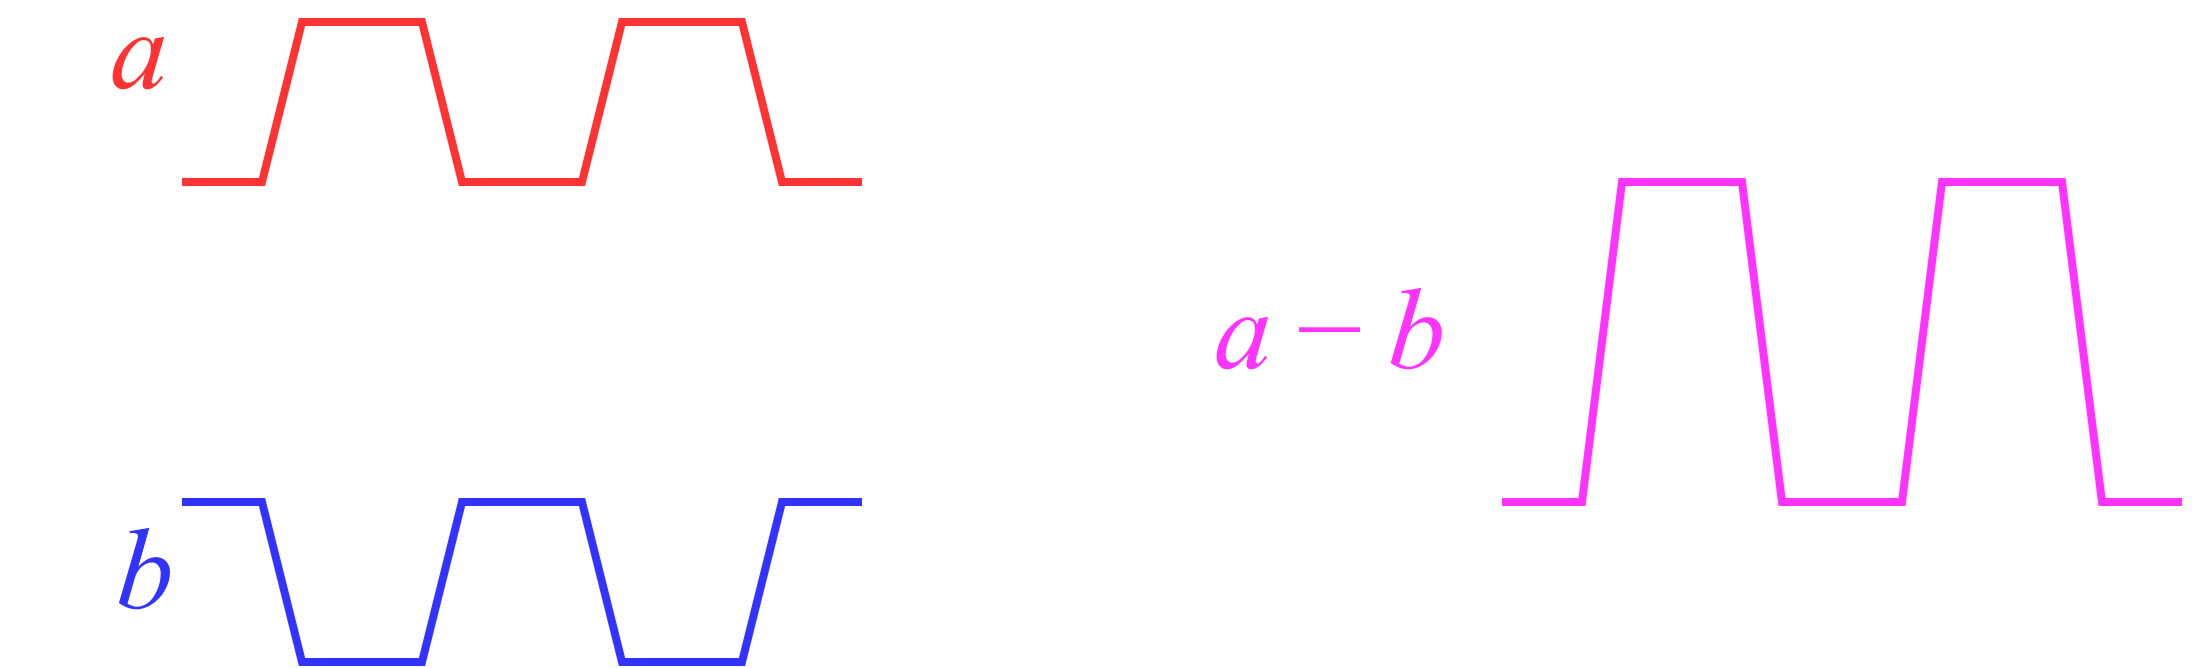
\includegraphics[width=.75\textwidth]{media/diffsig.png}
    \caption{Differential signalling illustrated. The signal is the difference between the signals on line $a$ and $b$.}
    \label{fig:diffsig}
\end{figure}

